\documentclass{article}
\usepackage{amsmath}
\usepackage{amssymb}
\usepackage{graphicx}
\title{Homework 3, 601.465 - Natural Language Processing}
\author{Matthew Jo}
\date{October 12, 2025}
\begin{document}

\maketitle

\textbf{1}

Using \texttt{switchboard-small}, the model's perplexity per word on each of the three sample files is as follows.
\begin{itemize}
	\item sample1: 230.8033
	\item sample2: 316.5347
	\item sample3: 313.0219
\end{itemize}

Using \texttt{switchboard}, the model's perplexity per word on each of the three sample files is as follows.
\begin{itemize}
	\item sample1: 280.4034
	\item sample2: 369.4896
	\item sample3: 456.3510
\end{itemize}

Log2-probabilities decrease and perplexities increase if I train on the larger \texttt{switchboard} corpus. It is because the larger corpus covers more vocabulary, reducing the number of instances of OOV while reading the sample texts. Since OOV is a placeholder for \textit{all} words outside of the vocabulary, it results in having higher probability (and thus lower perplexity) than other words.

\pagebreak

\textbf{3(a)} 69 out of 270 files were classified incorrectly. The total error rate is about $0.2556$. \\

\textbf{3(c)} \texttt{textcat} classifies all the dev files as \texttt{spam} when the prior probability of \texttt{gen} is $10^{-324}$. When it is $10^{-323}$, some dev files are classified as \texttt{gen}. \\

\textbf{3(d)} On the \texttt{gen} dev files, the minimum cross-entropy per token that I can achieve is $9.04616$ bits, when $\lambda = 0.005$. On the \texttt{spam} dev files, the minimum cross-entropy per token that I can achieve is $9.09572$ bits, when $\lambda = 0.005$. \\

\textbf{3(e)} The minimum cross-entropy per token that I can achieve on all development files together, if both models are smoothed with the same $\lambda$-value, is $9.06840$ bits, when $\lambda^* = 0.005$. \\

\textbf{3(f)} As shown in the graph below, at $\lambda = 0.005$, there is no obvious relationship between the length of a file and its cross-entropy per token. Performance tends to be divergent for short files, and it converges to a high cross-entropy as the file gets longer. \\

\begin{figure}[!h]
	\caption{Performance of add-0.005 on dev data for different file lengths (lowess smoothing, frac=0.666..., it=3)}
	\centering
	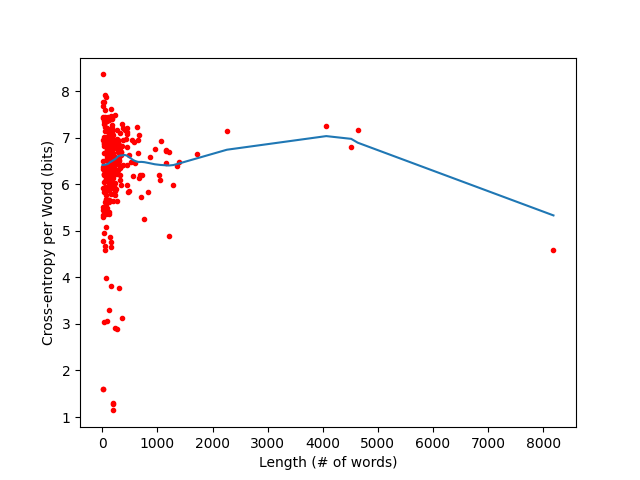
\includegraphics[width=\textwidth]{3f}
\end{figure}

\textbf{3(h)} I expect error rate to approach $0$ as training size approaches $\infty$. \\

\begin{figure}[!h]
	\caption{Performance of add-0.005 on dev data for different sizes of training data}
	\centering
	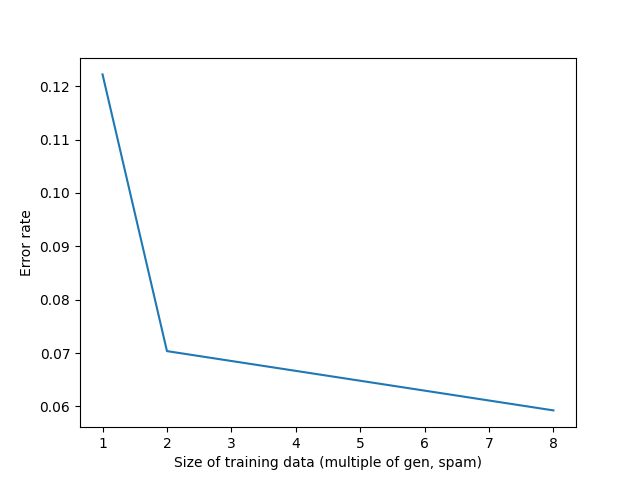
\includegraphics[width=\textwidth]{3h}
\end{figure}

\pagebreak

\textbf{4(a)} If I mistakenly took $V = 19999$ when there are $19999$ different word types in training data, both the uniform estimate and the add-$\lambda$ estimate can face a problem. For both cases, the sum of probabilities of all vocabularies would exceed $1$.

\begin{align*}
	\text{Uniform:} \qquad \sum_{i=1}^{19999} \frac{1}{19999} + \frac{1}{19999} (\text{OOV}) &= \frac{20000}{19999} \\
	\text{add-$\lambda$:} \qquad \sum_{i=1}^{19999} \frac{c(xyv_i) + \lambda}{c(xy) + 19999\lambda} + \frac{\lambda}{c(xy) + 19999\lambda} (\text{OOV}) &= \frac{c(xy) + 20000\lambda}{c(xy) + 19999\lambda}
\end{align*}

\textbf{4(b)} If $\lambda=0$, the add-$\lambda$ estimate would yield cross-entropy of $\infty$, since unseen words will yield the probability of $0$, and their log-value will be $-\infty$. \\

\textbf{4(c)} Suppose that $c(xyz) = c(xyz') = 0$.

\begin{align*}
	\hat{p}(z | xy) &= \frac{c(xyz) + \lambda V \cdot \hat{p}(z | y)}{c(xy) + \lambda V} \\
	&= \frac{c(xyz) + \lambda V \cdot \frac{c(yz) + \lambda V \cdot \hat{p}(z)}{c(y) + \lambda V}}{c(xy) + \lambda V} \\
	&= \frac{c(xyz) + \lambda V \cdot \frac{c(yz) + \lambda V \cdot \frac{c(z) + \lambda}{\sum_v c(v) + \lambda V}}{c(y) + \lambda V}}{c(xy) + \lambda V} \\
	\hat{p}(z' | xy) &= \frac{c(xyz') + \lambda V \cdot \frac{c(yz') + \lambda V \cdot \frac{c(z') + \lambda}{\sum_v c(v) + \lambda V}}{c(y) + \lambda V}}{c(xy) + \lambda V}
\end{align*}

It does not follow that $\hat{p}(z | xy) = \hat{p}(z' | xy)$. Even though the trigram counts are equal, the counts for the bigrams $yz$/$yz'$ and unigrams $z$/$z'$ may differ.

If, instead, $c(xyz) = c(xyz') = 1$, the answer is the same. Even though the trigrams are found in the training corpus, backoff still affects the overall estimated probability, so there is no guarantee that $\hat{p}(z | xy) = \hat{p}(z' | xy)$. \\

\textbf{4(d)} In add-$\lambda$ smoothing with backoff, increasing $\lambda$ increases the influence of the backoff probabilities to the probability estimates. Higher $\lambda$ results in the probability estimate being closer to the backoff probabilities based on the bigram and unigram counts.

\pagebreak

\textbf{6} I generated sentences with two models: \texttt{gen\_8\_0.005.model} and \texttt{gen\_5.model}. \\

\texttt{gen\_8\_0.005.model}:
\begin{itemize}
	\item SUBJECT: Re : \&NAME \&NAME \&NAME : The \&NAME younger skills me moping Everybody blue revealed parts connector wondering filling
	\item SUBJECT: Re : \&NAME \&NAME Avenue hair heart NOTICE cunning lot practices retainer Repeat drinks dirty income r\_a work-filled ONLY
	\item SUBJECT: Re : \&NAME ] - editing challenge nearby parted teaching + THIS own non-returnable treats scheme he weighing Director
	\item SUBJECT: \&NUM \&NAME : \&EMAIL <END\_QUOTE> Me obviously shirts Everybody Of hundreds fee password overview was visiting top\_docs hotmail single
	\item SUBJECT: Re : ? resources wear KNOW third People games perfect Below cuz drink Body AntoineIce present replying Incidentally including
	\item SUBJECT: Re : To issued folders believe hand In process sarcastic action electronic phones exercise Helpers volunteers occupation result Independence
	\item SUBJECT: OOV \&NAME \&CHAR any price House backup decided quite offer caused customer mind several huge captain affiliates Address sincerely
	\item SUBJECT: where alert replies involed reception visitors poster OVERALL Safety sick ever FOR Hop-on ie with indicate records sarcastic institutions
	\item SUBJECT: \&NAME OOV OOV . \&NAME \&NAME : ( \&NUM : \&NUM ) \&NUM \&NAME \&CHAR , \&NAME and present
	\item SUBJECT: reminder traditional Independence finish AT relevant muscles You mortgage record chance ha took Event unintelligible wrong hard death For
\end{itemize}

\texttt{gen\_5.model}:
\begin{itemize}
	\item nearby matters old hour Science pm Okay continue <QUOTE> getting bill developed updates auld triples or French eval main offer
	\item year upon forwards convenient nothing modern credit pricing 26th \&SMILEY factory assume Inc. rock include Event led fields task pre-varsity
	\item given between Evil respirators Make Are account months regret representation space audible advance promise awesome Dialogue supplies nicety miss identified
	\item appeal discourse economics permission break HILLSIDE conference last reasonable Hello realised chips photos anyway group booked HI call 'Stop choose
	\item time torture industry displayed awesome language If avoid job be Find lack Further huge hear quest just length x informatin
	\item clean November preference monsignor behavior FOR monsignor green approval feedback drive colleagues quality Acoustic never photograph candidate races beyond award
	\item waste Events Turn lesser tomorrow separate minerals psychologist +Do opt Dollars construct events elitist darn wo today Back yourself queries
	\item include Under \# Inc. Unless aging lesser problem sleep nltools 1500m also imminent href' lasting event event differences afraid photo
	\item products mood External OF brief Smallest amusing tobacco expected relational finish Unless Upon disclose important saturday Citrate You Very slip
	\item wish trip applies forwarding masks President consist System younger base pictures purchased i.e. off Get check themselves writing watch door
\end{itemize}

One striking difference is that the former model generates sentences that start with "SUBJECT" whereas the latter model does not. It is because the latter model has a very high lambda value which gives less weight to the most probable word.

\pagebreak

\textbf{7(c)}

\end{document}








































